\section{Discussion}
%%%%%%%%%%%%%%%%%%%%%%%%%%%%%%%%%%%%%%%%%%%%%%%%%%%%%%%%%%%%%%%%%%%%%%%%%%%%%%%
Using the forward-JWKB approximation we obtained three sets of results: amplitudes in $D = 3$ with massless mediation, amplitudes in $D = 4$ with massless mediation, and amplitudes in $D = 3$ and $D = 5$ with massive mediation.

In $D = 4$ with massless mediation, we found forward-JWKB amplitudes (\ref{AHN4}) for mediating quanta with spin $0$, $1$ and $2$. Each of these amplitudes exhibits an infinite number of singularities that lie outside of the physical scattering region. Indeed, the singularities (\ref{sJ0}), (\ref{sJ1}) and (\ref{sJ2}) agree with the two-body bound-state energies found in \cite{BIZJ,KabatOrtiz,Dittrich}. Upon taking the static limit ($m_{1} / m_{2} \rightarrow 0$), the resulting one-body amplitudes agree with those found in \cite{Singh} by solving one-body field equations. All of these amplitudes display an exponentiated divergent contribution, the kinematic dependence of which agrees with those found in \cite{Weinberg:1965nx} due to infrared photons and gravitons. Inside the physical scattering region, the coefficient of this divergence is imaginary and thus the whole divergence appears as a pure phase factor. This guarantees that physical observables are finite.

From the discussion in \S\ref{sec2} it should be clear that the Regge regime and the forward-JWKB regime are very different. The amplitude (\ref{AHN4}) in $D = 4$ exhibits Regge behavior with leading Regge trajectory function
\begin{equation}
	R_{N}(s) = -1 + \alpha_{N} \rho_{N}(s);
\end{equation}
and daughter trajectories $R_{N}(s) - l$. In Figure \ref{fig012} we plot the forward-JWKB leading Regge trajectories for $N = 0$, $1$ and $2$ as functions of the dimensionless variable
\begin{equation}
	\xi(s) \equiv \frac{s - M_{1}^{2} - M_{2}^{2}}{2 M_{1} M_{2}} \approx \frac{s - m_{1}^{2} - m_{2}^{2}}{2 m_{1} m_{2}}.
\end{equation}

\begin{figure}
\centering
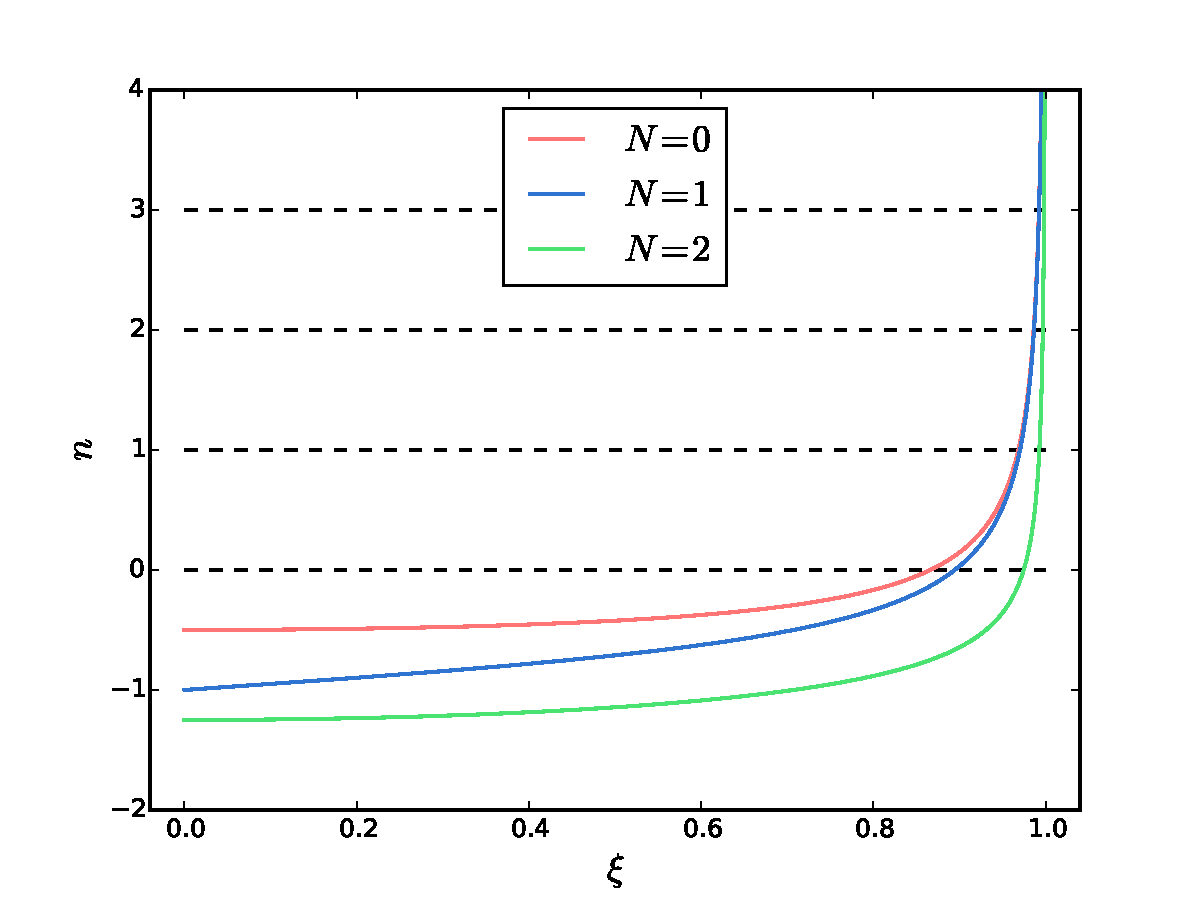
\includegraphics[scale=0.56]{figures/012.pdf}
\caption{The leading Regge trajectory functions $R_{N}(\xi)$ for spin $N = 0$, $1$ and $2$ in the forward-JWKB regime. The dashed lines correspond to integer values of $n$. For the couplings we have used $\alpha_{0} / (M_{1} M_{2}) = 0.5$, $Z_{1} Z_{2} \alpha_{1} = -0.5$, and $M_{1} M_{2} \alpha_{2} = 0.5$.}
\label{fig012}
\end{figure}

\begin{figure}
\centering
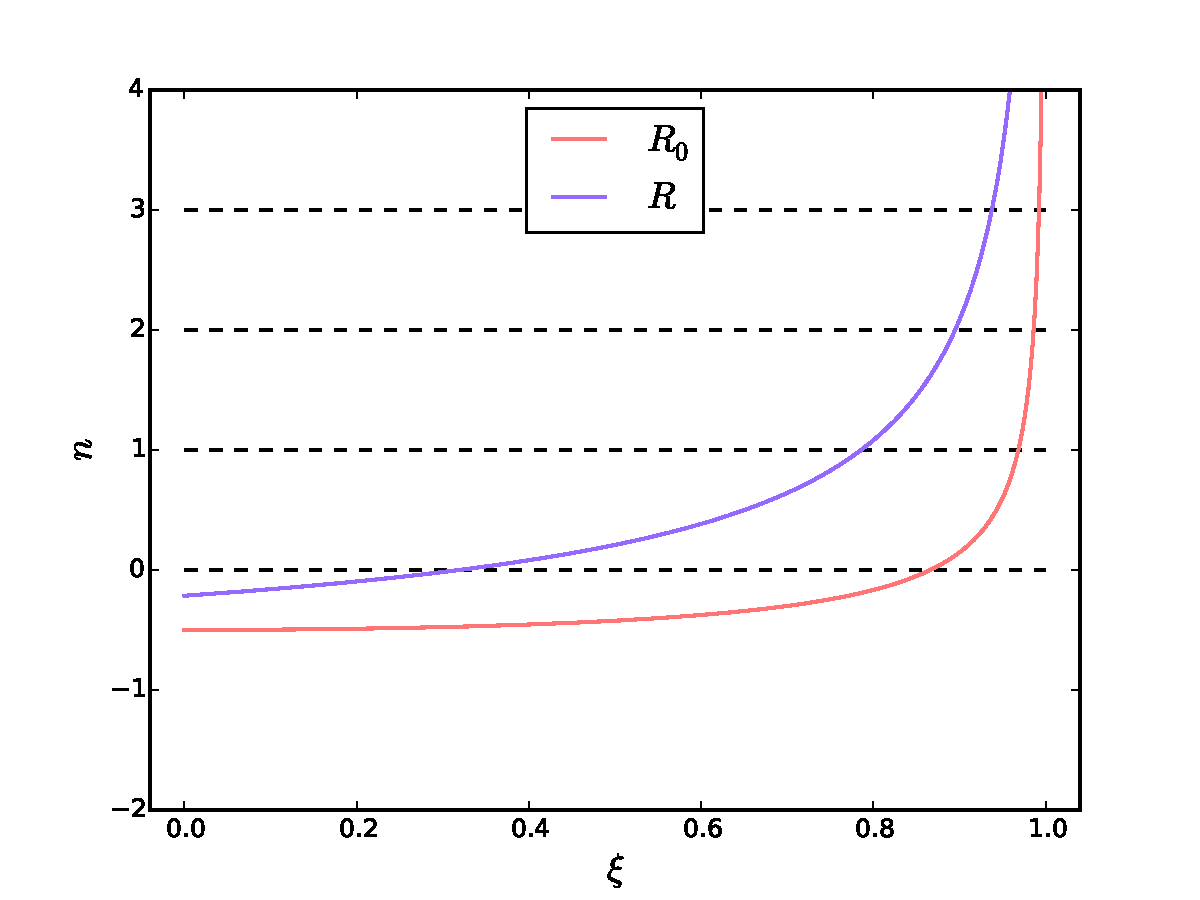
\includegraphics[scale=0.56]{figures/R0R.pdf}
\caption{The leading Regge trajectory for an interaction mediated by a massless scalar in the Regge limit ($R$) and the forward-JWKB regime ($R_{0}$).}
\label{figR0R}
\end{figure}

When $N = 0$ the forward-JWKB leading Regge trajectory $R_{0}$ is qualitatively different from the leading Regge trajectory function $R$ found in the Regge limit (\ref{ladders}). In Figure \ref{figR0R} we compare the leading trajectory in these two regimes. This comparison is only qualitative, as the normalization of the coupling strength $g$ in the Regge ladder sum (\ref{ladders}) is not necessarily the same as the one we used in the forward-JWKB amplitude. One major difference is that the real part of the Regge limit trajectory $R$ is non-vanishing in the region $\xi < 1$, while the real part of the forward-JWKB trajectory $R_{0}$ is non-vanishing in the smaller interval $-1 < \xi < 1$. However, near the threshold value both trajectories agree. Indeed, the discrepancy between these two trajectories was already noticed in \cite{Levy:1970yn}, where diagrammatic methods were used to sum over ladder contributions. Looking at the equations for $\rho$ in (\ref{LeeSawyer}) and $\rho_{0}$ in (\ref{rho0D4}) we see that the logarithm term in $\rho$ is missing from $\rho_{0}$. This logarithm term is proportional to the sum of the rapidities of the incoming states (\ref{rap12}), and is kept fixed in both the Regge and forward-JWKB limits. In future work we hope to address this shortcoming.

The forward-JWKB result (\ref{AHN4}) includes a factor involving an Euler Gamma function that is missing from the Regge limit ladder result (\ref{ladders}). A similar factor can be obtained using the Bethe-Salpeter equation \cite{LeeSawyer}. In order to obtain such a factor from field theory, one can use the Mellin transform technique \cite{BjorkenWu,TruemanYao} on the sum over ladder diagrams \cite{Polkinghorne1,Polkinghorne2} which helps to pick out non-leading logarithmic contributions.

The forward-JWKB amplitude in $D = 3$ with massless mediation exhibits the familiar tree-level singularity near $t = 0$, and also an ``extra'' non-perturbative singularity at a particular value $s = s_{*}(t_{*})$ that depends explicitly on $t_{*}$. For mediating scalars and photons, the location of the extra singularity is very similar to the location of the corresponding two-body bound state energies $s_{nl}$ in $D = 4$. Indeed, one can ``switch'' between the many singularities $s_{nl}$ and the one singularity $s_{*}$ with the replacement
\begin{equation}
	\frac{2 \pi \beta^{2}_{N}}{t_{*}} \longleftrightarrow \frac{\alpha^{2}_{N}}{(n + l + 1)^{2}};
	\label{74}
\end{equation}
where $\beta_{N}$ is the coupling in $D = 3$, and $\alpha_{N}$ is the coupling in $D = 4$. Upon analytic continuation to spin $2$, we also find a forward-JWKB amplitude with two singularities. However, unlike the scalar or photon cases, the $s_{*}$ singularity does not seem to correspond to anything that can be built with perturbative contributions (i.e. from contributions that are proportional to positive integer powers of the coupling). Unlike the $D = 4$ singularities $s_{nl}$, we seem to always be able to move the $D = 3$ singularity $s_{*}$ to the interior of the physical scattering region by allowing $t_{*}$ to be negative. Of course, the relation (\ref{74}) only holds when $t_{*}$ is positive.

We also studied the mediation of a heavy scalar in $D = 3$. In this case we found a non-perturbative expression that agrees with the expected result from adding forward-JWKB ladder diagrams of the form (\ref{fJWKBBox}) and (\ref{fJWKBDoubleBox}). Due to the particular details of the long-distance propagator in $D - 2 = 1$ dimensions, the result can be written as a sum of simple poles at the multi-mass values $(L+1)^{2}M^{2}$. The end result (\ref{615}) takes a very simple form that is analogous to Regge behavior, but instead of Regge poles along the $s$ axis, we find poles along the $t$ axis.

Then, instead of turning to $D = 4$ with a heavy mediator, we turned to $D = 5$. The reason for this is that when $D = 5$ we have $D - 2 = 3$ which is the other instance when the long-distance propagator is exact. Although we cannot evaluate the ``eikonal'' integral (\ref{DAvarphi}) exactly, after a series expansion we recover the familiar tree-level amplitude, a finite one-loop contribution and divergent higher-loop contributions. This system in $D = 5$ was considered mostly to illustrate that for higher-dimensional systems one can apply the forward-JWKB approximation and obtain limited results for all-order amplitudes.

In our calculation of forward-JWKB amplitudes we neglected the part of the forward Van Vleck matrix with derivatives of $\Sigma_{\text{two}}$ (the term with two-body interactions). The Van Vleck determinant is the first-order JWKB contribution. When written in the form (\ref{sqrtV}), it is clear that this contribution involves an infinite set of perturbative contributions (i.e. involving powers of the coupling). This demonstrates nicely the non-perturbative nature of the JWKB approximation. In principle, incorporating the contributions from $W$ in (\ref{sqrtV}) offers a way to go beyond the familiar $D = 4$ results obtained in this work. However, in practice it is not clear at the moment how to then evaluate the integrals in $\mathcal{S}_{T}$ and find the amplitude.

At first glance, the statement of the forward-JWKB approximation (\ref{fJWKBLimit}) amounts to a restriction on kinematics. But as was found in \cite{HalpernSiegel}, the semiclassical approximation has dynamical consequences that depend on the number of spacetime dimensions. Indeed, we found that in $D = 3$ the forward-JWKB approximation was consistent with weak couplings $\beta_{N}$, but in $D = 4$ we require strong couplings $\alpha_{N}$ when the quantum number becomes large. This strong-coupling feature is attractive and one hopes to be able to extend it to other theories (or at least to higher-point forward-JWKB scattering). It is also one of the reasons why we believe semiclassical first-quantized methods are important and useful to obtain non-perturbative results.